\documentclass{article}
\usepackage[utf8]{inputenc}
\usepackage{graphicx}
\usepackage{setspace}
\usepackage[top=1in,bottom=1in,left=1in,right=1in]{geometry}
\usepackage{amssymb}% http://ctan.org/pkg/amssymb
\usepackage{pifont}% http://ctan.org/pkg/pifont
\newcommand{\cmark}{\ding{51}}%
\newcommand{\xmark}{\ding{55}}%


\title{CS51 Final Project \\ \large Extensions}
\date{May 2019}

\begin{document}

\maketitle

\section{Introduction}
I decided to extend my program by including lexically scoped environment semantics and a unit expression type. I initially tried to implement type checking for the branches of conditional statements, but soon realized that the problem was much more difficult than it seemed. Without type inference, I would have to evaluate each branch of the conditional and check that the outputs were of the same type. But, if, for example, the conditional statement is part of a recursive function, the attempt to evaluate both branches could result in stack overflow. So this problem reduced to implementing type inferencing, so decided to do different extensions, which I will describe below.

\section{Lexically scoped environment semantics}
For all of the expressions in which no variables are bound in their evaluation, I was able to abstract away their outputs into a function I called ``abstracted\_eval," which takes as inputs the evaluation function (which is defined based on a particular scoping), an expression, and the environment. In particular, the functionality for numbers, booleans, unary operators, conditionals, raises,
binary operators, the Unassigned type and the Unit type, did not differ drastically (except for in the ways their arguments were evaluated), so the evaluation of these expressions in themselves does not involve binding any variables. Thus, for my lexical evaluator, I only defined unique outputs for functions, variables, let statements, recursive let statements, and function applications. I will describe how I handled each of these cases in the subsections below. 

I also want to note that I adapted my unit tests to check for the correct outputs for eval\_l, which is demonstrated in the file ``evaluation\_tests.ml." For example, the following example in the textbook (which I included in my unit tests) results in different outputs with dynamically versus lexically scoped environment semantics:

\begin{figure}[ht]
\begin{center}
\includegraphics[width=.25\textwidth]{book_ex1.png}
\end{center}
\caption{This function evaluates to 5 under dynamic semantics, but it evaluates to 4 under lexical semantics and substitution semantics.}
\end{figure}

\subsection{Variables}

The value assigned to a variable is stored in the environment. So the evaluation of a variable involves looking up its value in the environment. Because variables are not functions, they are treated the same way in dynamic and lexical scoping. If the variable is not assigned to a value in the given environment, then my lookup function in the Env module returns an EvalError. 

\begin{figure}[ht]
\begin{center}
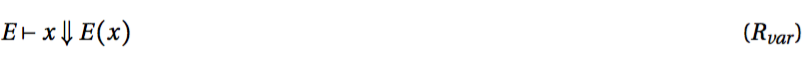
\includegraphics[width=.7\textwidth]{var_lex.png}
\end{center}
\caption{Textbook lexical environment semantic rule for variables.}
\end{figure}

\subsection{Functions}

\begin{figure}[h]
\begin{center}
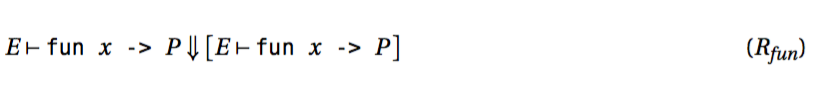
\includegraphics[width=.7\textwidth]{fun_lex.png}
\end{center}
\caption{Textbook lexical environment semantic rule for functions.}
\end{figure}

As an adaptation from the dynamic evaluator, the lexical evaluator returns a closure, which contains both the function and the environment in which it is defined. This is because in lexical scoping, variables are defined based on the environment the function is defined in, where in dynamic scoping variables are defined based on the environment the function is applied in.

\subsection{Let statements}

\begin{figure}[h]
\begin{center}
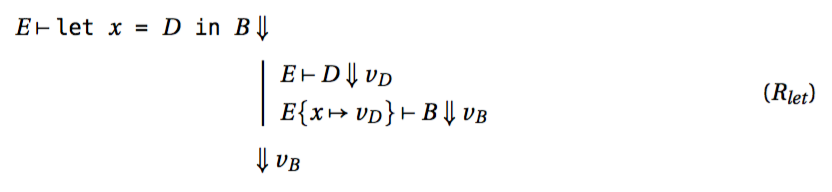
\includegraphics[width=.7\textwidth]{let_lex.png}
\end{center}
\caption{Textbook lexical environment semantic rule for let statements.}
\end{figure}

The evaluation of let statements does not differ between dynamic and lexical scoping, except for the fact that we recursively call eval\_l in lexical scoping (rather than eval\_d) on the body of the statement. We simply evaluate the body of the let statement in the environment, extended so that the first argument of the let statement (of type varid) maps to the given value.

\subsection{Recursive let statements}
We need to first evaluate the defintion in the letrec expression in an environment where the first argument of the letrec statement (call it $x$), is mapped to this Unassigned expression. But after we have evaluated the definition, we need to evaluate the body where $x$ is no longer mapped to Unassigned. In order to map $x$ to the output of evaluating the definition, we need to initially store the Unassigned expression in some location, and then reassign the value stored at that location using references. Without using references, the value for $x$ will not get reassigned, as the pointer will not move and what is stored in the reference will not be changed, and thus the Unassigned expression will remain in the environment. 

We next find the output of evaluating the body in the environment where $x$ is mapped to the result of evaluating the definition (phew!). Finally, we match this output with an Unassigned value or any other value type. If it is Unassigned, this means that when we mapped $x$ to the result of evaluating the definition, ``Unassigned" was contained in this result. This could only if there is infinite recursion in the statement, such as 

$$ \textbf{let rec  } x = x \textbf{ in } x $$

because the value of $x$ relies on the value of $x$ in the definition and vise versa. Thus we raise an EvalError if the return type is an Unassigned value, otherwise we return whatever was outputted by the evaluation.

\begin{figure}[h]
\begin{center}
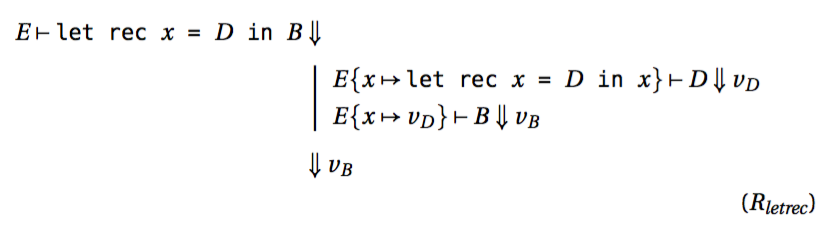
\includegraphics[width=.7\textwidth]{letrec_lex.png}
\end{center}
\caption{Textbook lexical environment semantic rule for recursive let statements.}
\end{figure}



\subsection{Function applications}

\begin{figure}[h]
\begin{center}
\includegraphics[width=.7\textwidth]{app_lex.png}
\end{center}
\caption{Textbook lexical environment semantic rule for function applications.}
\end{figure}

First we evaluate the two arguments in the application. The first must be a function, and the second can be of any type. We check that the first evaluation outputs a function using a match case. If it is a closure containing a function and an environment, then we evaluate the body of that function with the environment from the closure extended so that the variable bound by the function maps to the value given as the second argument in the application. Otherwise, we return an EvalError. In this way, we are using lexical scoping, as we evaluate the function application based on the environment it was defined in rather the environment it is being applied in. 


\section{Adding a unit expression type}
I chose, as an extension, to add a ``unit" component to the expression algebraic data type. Examining the documentation for the OCaml language, a ``unit" is not included under the list of atomic types. I assume this is because a unit communicates no information, and is unique in this way. Units can be useful when, for example, one wants their program to produce a side effect but directly return no value, or when constructing for or while loops, or when one wants to create a function that requires no inputted values. Although some of these reasons for the unit type are not yet possible in my simple implementation of the OCaml language, the unit type would be essential if my code was expanded upon.

Implementing the unit type involved editing the following files:

\begin{itemize}
    \item expr.mli
    \item expr.ml
    \item evaluation.ml
    \item evalution\_tests.ml
    \item miniml\_parse.mly
    \item miniml\_lex.mll

\end{itemize}

I will now describe my edits to each of these files. 

\subsection{Edited files}

\subsubsection{expr.mli}
I added a ``Unit" type to the algebraic data structure for expressions. Unit takes no arguments, as it returns nothing and is applied to nothing.

\subsubsection{expr.ml}
There are no free variables in a unit, so free\_vars returns an empty variable set when applied to a Unit. For this reason, subst simply returns the Unit when applied to the Unit (no free variables). A unit is expressed as a concrete string like so: (). Finally, Unit as an abstract string is simply a string containing the word Unit like so: ``Unit".

\subsection{evaluation.ml}
The outcome should be the same evaluating a Unit using any semantics: a Unit should be returned. So this is what I did for all of the evaluation functions I created, namely

$$\textbf{Unit } -> \textbf{Env.Val Unit}$$

\subsubsection{evaluation\_tests.ml}
I tested that a the evaluation of a Unit always results in a Unit. I also checked to be sure that the unit type worked as an input and output for functions.

\subsubsection{miniml\_parse.mly}
I added UNIT to the token structure. 

\subsubsection{miniml\_lex.mll}
I used the following website as a refernce to understand this file: \\
https://caml.inria.fr/pub/docs/manual-ocaml/lexyacc.html. 

I added the UNIT token to the symbol hash table, associating the Unit with the symbol (). I also added the Unit symbol to the ``sym" construct as follows:

\begin{figure}[h]
\begin{center}
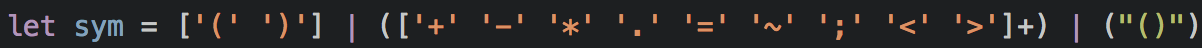
\includegraphics[width=.7\textwidth]{sym.png}
\end{center}
\caption{The ``sym" construct in miniml\_lex.ml.}
\end{figure}

The rightmost symbol was my addition for the Unit. In accordance with the syntax from the above url, I enclosed the symbol for the unit in parentheses, as the inputted string should match that one exactly to match to the unit type, e.g. ``)(" should not match to the unit type. This is the syntax for indicated the exact string must be matched.

\subsection{Limitations}
One key limitation in my implementation of the Unit type that I did not get to addressing is the fact that Unit currently cannot be used as an input to a function in an expression, unless formatted as a string, e.g.

$$\textbf{Fun(``()", Var}(x)\textbf{)  \checkmark} $$

works but

$$\textbf{Fun(Unit, Var}(x)\textbf{)  \xmark}$$

is considered mistyped. This is because the Fun construct is defined as taking in a tuple whose first argument is a varid, and a Unit is of type expr. Thus the definition of a function would have to be changed in order to resolve this issue.


\end{document}
